\chapter{Results and Discussion}

This purpose of this chapter is to describe the testing prodecures, results, and implementation issues that were encountered during the implementation phase of the project. Whenever possible, concrete results will be compared with those described previously in Ch.\ \ref{cha:goals}.

The Engine and Transmission, and Braking modules both require that the Formula SAE 2010 vehicle be at least partly complete for testing. Since the build schedule for the vehicle is to have it complete for the beginning of May, 2010, much of the final-stage testing and tuning of these modules was not yet possible as of writing.

\section{CAN Transceiver Hardware Bug}

After the first module, the Engine and Transmission module, was populated, we proceeded to inspect all solder joints and check for shorts between VCC and ground. Initially no problems were apparent, but when we first applied power to the module, using a current limiting bench power supply, a dynamic short circuit quickly appeared. The power supply immediately began limiting current, and the voltage dropped.

After a lot of searching, inspecting all the components under a microscope, and hot air rework, it was determined that the problem was not with any of the solder joints or the PCB, but in fact a problem with the schematic. In error, the circuit design for the CAN Transceiver had got the VCC and GND lines to the chip swapped. Additionally, this CAN Transceiver schematic block had been duplicated to all four modules, which resulted in the same fate.

A fix was quickly implemented, first on the Engine and Transmission module, and subsequently for the other modules. The copper traces to the VCC and GND pins on the CAN Transceiver were cut with an exacto knife, and rewired correctly with wire-wrap wire.

\section{Transmission}

\subsection{Electro-pneumatic Simulation}

The electro-pneumatic Simulink model as described in Sec.\ \ref{sec:electropneumatic_implementation} was simulated by feeding the closed-loop system with a reference input representing 50\% of the maximum travel of the clutch. Figure \ref{fig:pneumatic_sim} shows the closed-loop response to the step input, recorded until the output stabilized. Figure \ref{fig:pneumatic_sim_zoom} shows a close up view of the first peak in the response, detailing the result of the compressibility effects of the air in the cylinder. The PID controller block was minimally tuned only until a stable response was obtained.

\begin{figure}[htp]
 \centering
 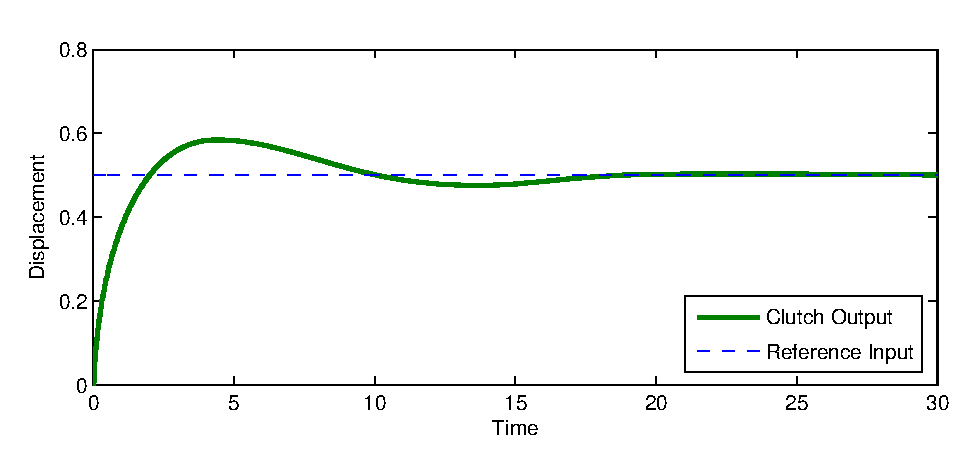
\includegraphics[width=6in,keepaspectratio]{results/figures/electro-pneumatic_simulation_plot.eps}
 \caption{Output from Simulink electro-pneumatic model}
 \label{fig:pneumatic_sim}
\end{figure}

The point of the simulation was to verify the feasability of closed-loop control over the electro-pneumatic system in the configuration proposed. It is important to note that correct model parameters corresponding to the real physical pneumatic valves, cylinders, clutch, etc., were not obtained.

\begin{figure}[htp]
 \centering
 \includegraphics[width=6in,keepaspectratio]{results/figures/electro-pneumatic_simulation_plot2.eps}
 \caption{Close-up of the first peak in Fig. \ref{fig:pneumatic_sim}}
 \label{fig:pneumatic_sim_zoom}
\end{figure}


\subsection{System testing}

Since testing and tuning of the full electro-pneumatic system requires that the 2010 Formula SAE vehicle be complete, this phase of the project was not completed as intended, and is recommended for future work.


\section{Intake}


\section{Braking}


\subsection{Bias Adjustment}


\subsection{Calibration}


\section{Telemetry}

The electronic hardware for the driver interface module was completely constructed and debugged. Additionally, all low-level drivers and system software were completed. Successful transmission tests were conducted between the telemetry module, ECU, DAQ, and a laptop running the software for the ECU and DAQ.

Getting the software implementation of the telemetry module to work successfully was far more difficult than originally imagined. The individual components of the system software would run as expected on their own, but fail when coupled together. For example, the ECU data link and the DAQ data link were at one point in the software development process relatively stable in operation by themselves, but enabling both would cause data loss, or one of the two links to drop. A large amount of time was invested in investigating the causes of these problems, and will be discussed in this section.

\subsection{Wireless Data Link}

We had originally planned to run the wireless link's data rate higher than \unit{115.2}{\kilo\bit\per\second}. The XBee documentation states that the modem is capable of running up to \unit{250}{\kilo\bit\per\second}, and the XBee modems allow for a continuous range of baud rates to be selected. Unfortunately it was determined that the XBee Pro can not set it's baud rate to \unit{230.4}{\kilo\bit\per\second}, which is the highest possible baud rate supported by the MAX3100.

The MAX3100 was therefore configured to operate at \unit{115.2}{\kilo\bit\per\second}, and the XBee modem's interface rate was matched. A simple throughput stress test was performed that continuously wrote data in 16 byte chunks into the MAX3100's driver's software transmit buffer. A fixed-length 32 byte software buffer was never overrun with this test, and an actual data throughput of $\unit{8.251}{\kilo\byte\per\second}$ was observed with a logic analyzer on the TX pin of the MAX3100.

The range of the modems was not tested. Since the output power of the telemetry module's transmitter depends on the antenna and how it is mounted on the car, this will need to be tested after the car has been built in order to verify that this design improves upon the previous generation.

\subsection{Wireless Link Bench Testing}

Simultaneous data streams from both the DAQ and ECU were successfully bench tested using two separate end modems connected to the same laptop. The laptop, running Ubuntu Linux, used Sun VirtualBox to host a session of Windows XP in order to run the proprietary ECU and DAQ software. Figure \ref{fig:telemetry_bench_test} shows the telemetry module being monitored with a logic analyzer, and communicating with another modem (the blue module on the right.)

\begin{figure}[H]
 \centering
 \includegraphics[width=5in,keepaspectratio]{results/figures/telemetry_module_test_bench.eps}
 \caption{Photograph of the telemetry module being debugged with a protocol analyzer.}
 \label{fig:telemetry_bench_test}
\end{figure}

The DAQ was configured to output all analog channels at a maximum of \unit{10}{\hertz} at an RS-232 baud rate of \unit{38}{\kilo\bit\per\second}, while the ECU was operated at a fixed \unit{57.6}{\kilo\bit\per\second}.

The ECU connection to the DTASWin software performed the same as with a hard line connection, and without any issues. The DAQ connection to the DAQ software on the PC worked without the software reporting any synchronization errors, but the refresh rate of the data was lower than expected. Inspection of the serial links in and out of the telemetry module with a logic analyzer confirmed the suspicion that not every packet received from the DAQ was being transmitted, however no corrupt or partial packets were being transmitted either.

Incoming data from the DAQ that the decoder is not able to decode is discarded. Seeing a large amount of discarded data, as we were, would indicate an issue with the DAQ library. This will be investigated further.

\subsubsection{DAQ Packet Injection}

Additionally, a second test was performed with the DAQ serial link by injecting data encoded on the telemetry module using the DAQ encoder. Every time a real incoming packet from the DAQ was decoded, it was forwarded along with an artificial one. This test proved successful, and the DAQ software was able to display the artificial ``analog'' channel, even though no such physical channel existed on the DAQ unit.



\section{Driver Interface}



%\subsection{Driver Controls}


%\subsection{Diagnostic Information}


\subsection{LCD Interface}

The memory-mapped LCD module interface, as described in \ref{sec:lcd_module_data_interface}, proved to be very useful in implementing the user interface software. By using GDB connected to the running Driver Interface module, it was possible to read and write data directly to the LCD by issuing GDB memory access commands. Several GDB macro scripts were set up

\subsubsection{Bench Experiments}

To verify the LCD data interface circuitry before the final Driver Interface module hardware had been completed, a bench test of the LCD module with an ARM7 development board was conducted. The bus interface as designed in Sec.\ \ref{sec:lcd_module_data_interface} was implemented on a breadboard: a latch and level shifter were used as in the Driver Interface module circuit design, and an FPC cable adapter was constructed with the aide of the tech shop to allow connecting the LCD module to the breadboard. The GPIO pins on the ARM7 development board (shown in red in Fig.\ \ref{fig:can_bench_test}) were used to bit-bang the data interface to the LCD. This test setup was used to write the initial LCD module code used in the final Driver Interface module implementation.

\begin{figure}[h!]
\centering
\subfigure[LCD Bench test]{
  \label{fig:lcd_bench_test}
  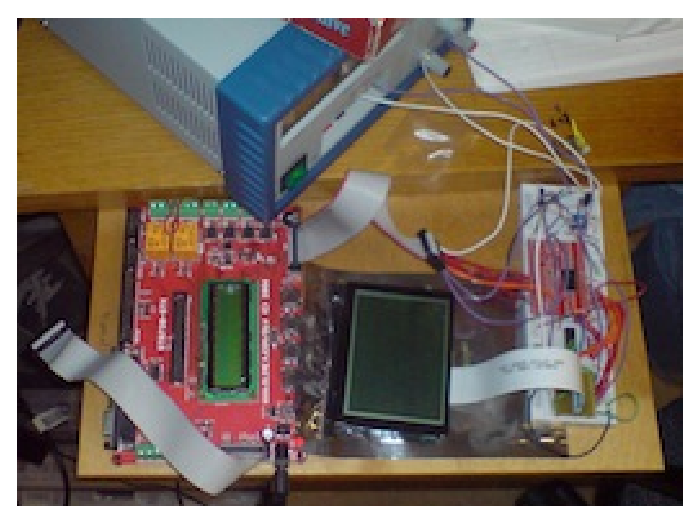
\includegraphics[width=2.5in,keepaspectratio]{results/figures/lcd_bench_test.eps}
}
\subfigure[CAN Bench test]{
  \label{fig:can_bench_test}
  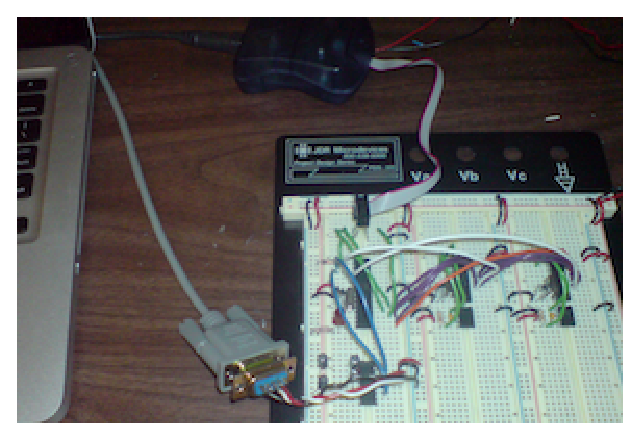
\includegraphics[width=2.5in,keepaspectratio]{results/figures/can_bench_test.eps}
}
\caption{Bench experiments conducted during the implementation phase.}
\label{fig:bench_experiments}
\end{figure}

\subsection{Graphics Display}

Once all the hardware bugs with the Driver Interface module had been corrected, it was possible to continue writing the LCD interfacing software that had been started during the initial LCD testing. The external memory interface circuitry described in Sec.\ \ref{sec:lcd_module_data_interface} worked without issue. Figure \ref{fig:driver_interface_lcd} shows the LCD displaying a sample bitmap from the manufacturer.

\begin{figure}[h!]
 \centering
 \includegraphics[width=6in,keepaspectratio]{results/figures/driver_interface_lcd.eps}
 \caption{Testing the LCD on the Driver Interface module.}
 \label{fig:driver_interface_lcd}
\end{figure}

\subsection{Vehicle Dynamic Adjustment}

\begin{figure}[h!]
 \centering
 \includegraphics[width=3in,keepaspectratio]{results/figures/driver_interface_menu.eps}
 \caption{Parameter menu on the Driver Interface module.}
 \label{fig:driver_interface_menu}
\end{figure}



\section{Implementation Issues Encountered}


\subsection{Hardware Implementation Issues}


\subsubsection{CAN Transciever Schematic Error}


\subsubsection{Driver Interface LCD Reset Line}


\subsubsection{Telemetry RS-232 Transciever Schematic Error}





\subsection{CAN Driver Problems}